%!TEX TS-program = xelatex
%!TEX encoding = UTF-8 Unicode

\documentclass[12pt]{extarticle}
% extarticle is like article but can handle 8pt, 9pt, 10pt, 11pt, 12pt, 14pt, 17pt, and 20pt text

\def \ititle {Origins of Mind}

\def \isubtitle {Lecture 01}

\def \iauthor {Stephen A. Butterfill}
\def \iemail{s.butterfill@warwick.ac.uk}
\date{}

%for strikethrough
\usepackage[normalem]{ulem}

\input{$HOME/Documents/submissions/preamble_steve_handout}

%\bibpunct{}{}{,}{s}{}{,}  %use superscript TICS style bib
%remove hanging indent for TICS style bib
%TODO doesnt work
\setlength{\bibhang}{0em}
%\setlength{\bibsep}{0.5em}


%itemize bullet should be dash
\renewcommand{\labelitemi}{$-$}

\begin{document}

\begin{multicols*}{3}

\setlength\footnotesep{1em}


\bibliographystyle{newapa} %apalike

%\maketitle
%\tableofcontents




%---------------
%--- start paste


\def \ititle {Lecture 09: Interaction in Radical Interpretation}

\begin{center}

{\Large

\textbf{\ititle}

}



\iemail %

\end{center}



\section{Radical Interpretation: The Question}

‘I want to know what it is about propositional thought---our beliefs, desires, intentions and speech---that makes it intelligible to others.’

\citep[p.~14]{Davidson:1995nl}


\section{The Intentional Stance}

‘the intentional stance ...

‘first you decide to treat the object whose behavior is to be predicted as a rational agent; ‘then you figure out what beliefs that agent ought to have , given its place in the world and its purpose. ‘Then you figure out what desires it ought to have, on the same considerations,
‘and finally you predict that this rational agent will act to further its goals in the light of its beliefs’
\citep[p.~17]{Dennett:1987sf}

‘one rule for attributing beliefs in the intentional strategy is this: attribute as beliefs all the truths relevant to the system's interests (or desires) that the system's experience to date has made available’ \citep[p.~18]{Dennett:1987sf}

‘We attribute the desires the system ought to have. That is the fundamental rule. It dictates, on a first pass, that we attribute the familiar list of highest, or most basic, desires to people: survival, absence of pain, food, comfort, procreation, entertainment.’ \citep[p.~20]{Dennett:1987sf}



\section{Social Cognition vs Radical Interpretation}

What is the relation between an account of radical interpretation
and a theory of social cognition?

‘Do people actually use this strategy? Yes, all the time.’
\citep[p.~21]{Dennett:1987sf}

‘[a]ll understanding of the speech  [and thoughts] of another involves radical interpretation’
\citep[p.~125]{Davidson:1973jx}

‘The approach ... I have outlined is not, I am sure it is clear, meant to throw any direct light on how in real life we come to understand each other’
\citep[p.~12]{Davidson:1980xp}

\citet[p.~22ff]{Marr:1982kx} distinguishes:

\begin{itemize}

\item computational description---What is the thing for and how does it achieve this?

\item representations and algorithms---How are the inputs and outputs represented, and how is the transformation accomplished?

\item hardware implementation---How are the representations and algorithms physically realised?

\end{itemize}

A theory of radical interpretation is supposed to provide
a computational description of social cognition.



\section{An Objection to the Intentional Stance}

Does the Intentional Stance actually describe how it would be possible,
even in principle, to infer facts about minds and actions from
evidence that can
be described without knowing anything about the particular actions, beliefs, desires and
other mental states of any individual?

No.  If an interpreter actually used Dennett’s Intentional Strategy,
what would enable her to distinguish your actions, beliefs, desires,
feelings and other mental states from anybody else’s?
Essentially only your location in space and your biological needs.
This is probably insufficient to distinguish
distinguish your actions, beliefs, desires, feelings and other mental
states from others nearby who have similiar biological needs.



\section{Davidson’s Theory of Radical Interpretation}

\begin{center}
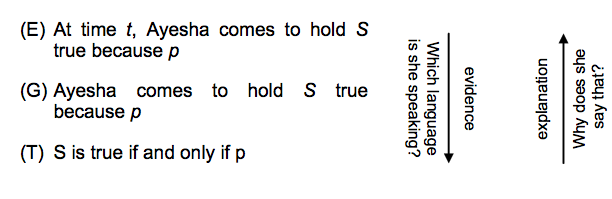
\includegraphics[scale=0.3]{img/radical_interpretation_handout.png}
\end{center}



\section{Objections to Davidson’s Theory of Radical Interpretation}

(1) No account of social cognition when the targets are wordless agents.

(2) No account of non-propositional mental phenomena, such as the unfolding of emotions.

1. On Radical Interpretation (and the Intentional Stance), the outputs of social cognition are (i) propositional attitude ascriptions and (ii) action predictions.

2. Emotions unfold ...

3. ... and this is not comprehensible as a series of changes in propositional attitudes.

So: 4. Understanding the way emotions unfold is not a matter of ascribing propositional attitudes or predicting actions.

But: 5. Humans do sometimes understand the way anothers’ emotions are unfolding.

So: 6. Radical Interpretation (and the Intentional Stance) is not a fully adequate computational description of human social cognition.


(3) Indeterminacy of reference

‘It makes no sense, on this approach, to complain that a theory comes up with
the right truth conditions time after time, but has the logical form
(or deep structure) wrong. We should take the same view of reference.’
\citep[p.~223]{Davidson:1977kn}

(4) A dilemma about The Evidence: actions or joint displacements

‘a radical interpreter is not, at the beginning of his study, informed about
any of the basic propositional attitudes of his subject.’
\citep[p.~17]{Davidson:1984pr}

‘The important limitation is that [the radical interpreter] doesn’t know in
detail the contents of any of the propositional attitudes of the person to
be interpreted: she doesn’t know what he intends, believes, wants or means
by what he says.’ \citep[p.~]{Davidson:1994ff}



\section{The Teleological Stance [recap]}

‘an action can be explained by a goal state if, and only if, it is seen as  the  most justifiable action towards that goal state that is available within the constraints of reality’
\citep[p.~255]{Csibra:1998cx}

‘Such calculations require detailed knowledge of biomechanical factors that
determine the motion capabilities and energy expenditure of agents. However,
in the absence of such knowledge, one can appeal to heuristics that approximate
the results of these calculations on the basis of knowledge in other domains
that is certainly available to young infants. For example, the length of
pathways can be assessed by geometrical calculations, taking also into
account some physical factors (like the impenetrability of solid objects).
Similarly, the fewer steps an action sequence takes, the less effort it might
require, and so infants’ numerical competence can also contribute to efficiency
evaluation.’ \citep{csibra:2013_teleological}



\section{Limits of The Teleological Stance}

The problem of opaque means:
failures to identify to which ends actions are means can impair goal ascription.

\emph{A Gricean circle}
communicative actions characteristically have  goals which the actions
are means to realising only because others recognise them as
means to realising those goals.



\section{Your goal is my goal}

An outcome is a \emph{collective goal} of two or more actions involving multiple agents
just if the actions are directed to this goal and this is not, or not just, a matter
of each action being individually directed to that goal.

\begin{enumerate}
\label{your_goal_is_my_goal}
\item You are
about to attempt to
engage in some joint action
or other with me.
%(for example, because you have made eye contact with me while I was in the middle of attempting to do something).

\item I am not about to change the single goal to which my actions will be directed.

\end{enumerate}
%
Therefore:
%
\begin{enumerate}[resume]
%
\item A goal of your actions will be my goal, the goal I now envisage that my actions will be directed to.
\end{enumerate}

Simple forms of interaction enable correct goal ascription in
situations where it would not otherwise be possible.
So if we are giving a computational description of
social cognition, we must consider the interpreter as not merely
observing her target but also potentially interacting with her.



\section{Interaction and Nonlinguistic Referential Communication}

1. At time t, Ayesha comes to hold ‘Questo è pericoloso’ true because p, while she is pointing to the dog

2. Something about the dog (and not, say, it’s Shoemaker shadow) explains Ayesha’s change in attitude towards  ‘Questo è pericoloso’.

Csibra’s ‘two stances’:

Teleological and referential action interpretation ‘rely on different kinds of action understanding.’
These are initially two distinct ‘action interpretation systems’ and they come together later in development
\citep[p.~456]{Csibra:2003kp}





%--- end paste
%---------------

\footnotesize
\bibliography{$HOME/endnote/phd_biblio}

\end{multicols*}

\end{document}
